\section{Precision time protocol}

Aunque el desarrollo del protocolo \gls{ntp} supuso un gran avance con respecto 
a las técnicas de sincronización en redes utilizadas anteriormente, la 
exactitud que podía alcanzar dicho protocolo no era suficiente para las 
aplicaciones con requisitos de altas prestaciones como los sistemas de control 
o sistemas de medición distribuidos. Para mejorar el rendimiento se propuso el 
desarrollo de un protocolo denominado \acrlong{ptp}, bajo el estándar 
\acrshort{ieee} 1588-2002 (año de su publicación) \cite{IEEE1588_2008}. 
Actualmente se utiliza la segunda revisión del estándar: IEEE 1588-2008 o 
\gls{ptp}v2, que no presenta compatibilidad con la versión anterior.

\subsection{Arquitectura de red}

El protocolo \gls{ptp} define una arquitectura jerárquica de tipo 
maestro-esclavo. Al igual que en la red \gls{ntp}, el nodo raíz puede estar 
conectado a una fuente estable de tiempo, como un \textit{\gls{gpsdo}} o un 
reloj 
atómico, y provee de sincronización al resto de la red. En el caso de \gls{ptp} 
este nodo recibe el nombre de \acrlong{gm}. Los nodos intermedios pueden actuar 
como maestros del nivel siguiente o como nodos finales. A continuación se 
detallan las características más relevantes de los tipos de dispositivos más 
usuales:

\begin{itemize}	
	\item \textbf{\gls{oc}} \\
	Este tipo de nodos se comunican con el resto de la red via una única 
	intefaz de red física de tipo bidireccional que se encarga del intercambio 
	de los paquetes con las marcas de tiempo con el resto de la red. La 
	configuración de \gls{oc} sólo permite una única ejecución del 
	protocolo 
	\gls{ptp} y un único estado de funcionamiento. Así, este tipo de 
	configuración, permite al dispositivo actuar como maestro de la red 
	(\acrshort{gm}) o como reloj esclavo.
	
	\item \textbf{\gls{bc}} \\
	Los dispositivos que actúan como \acrshort{bc} suelen disponer de múltiples 
	puertos físicos que pueden actuar como si fuesen \gls{oc}s pero que 
	comparten una misma referencia de tiempo (recuperada del nodo maestro en el 
	nivel superior). Es decir, uno de los puertos se configurará como esclavo y 
	el resto podrán actuar como puertos maestros para los siguientes nodos de 
	la red.
	
	\item \textbf{\gls{tc}} \\
	La gran diferencia con respecto a los tipos anteriores reside en que los 
	\gls{tc} no se sincronizan con un nodo maestro. Estos actúan como simples 
	repetidores del tráfico entrante, pero modifican el campo de corrección de 
	los mensajes \textit{Follow\_UP o Pdelay\_Resp\_Follow\_UP} para incluir el 
	tiempo de residencia de los paquetes \gls{ptp} en el \gls{tc}. El campo de 
	corrección es usado posteriormente por los \gls{oc} para realizar el ajuste 
	de su reloj interno. 
	Dependiendo del mecanismo empleado para el cálculo del tiempo de 
	propagación se distinguen dos tipos de \gls{tc}: \textit{End-to-end} y 
	\textit{Peer-to-peer}.
\end{itemize}

\subsection{Algoritmo}

En el protocolo \gls{ptp} se distinguen dos fases de ejecución:
\begin{enumerate}
	\item Establecimiento de la jerarquía en la red.
	\item Sincronización de los relojes.
\end{enumerate}

En el arranque del algoritmo \gls{ptp} se espera por un lapso de tiempo a 
recibir mensajes de tipo \textit{Announce} provenientes de algún maestro en la 
red. Si no se reciben mensajes de ese tipo, el nodo asume que es maestro hasta 
que un maestro con mejores prestaciones aparezca en la red. La configuración de 
roles en la red se realiza mediante un algoritmo llamado \gls{bmc}, que utiliza 
varios parámetros como calidad de la fuente de reloj de un nodo o el nivel en 
el que se encuentra de la jerarquía (entre otras cosas) para decidir quien debe 
actuar como maestro en la red y quien como esclavo. Este ordenamiento se 
realiza de forma dinámica, de manera que si un nodo se cae, el resto de la red 
se vuelve a configurar en base a los nodos supervivientes.

Tras la fase de establecimiento de la jeraquía se pasa a la fase de 
sincronización, basada en el intercambio de una serie de paquetes 
con marcas de tiempo que permiten al nodo esclavo el cálculo del desfase de su 
reloj con respecto al de referencia en el nodo maestro. El proceso se describe 
en la Figura \ref{fig:ptpts}:

\begin{enumerate}
	\item El maestro manda un mensaje de tipo \textit{Sync} que es sellado 
	temporalmente en base a la escala del maestro en el momento de su envío. 
	Este mensaje puede contener su marca temporal ($T_1$) o necesitar de otro 
	tipo de 
	mensaje (\textit{Follow\_Up}) para transmitirla.
	
	\item El esclavo anota el tiempo de recepción (en su propia escala de 
	tiempo) del mensaje en la marca $T_2$.
	
	\item El esclavo manda un mensaje de tipo \textit{Delay\_Req} al maestro y 
	almacena la marca de tiempo en que lo hace ($T_3$).
	
	\item El maestro sella la recepción del paquete recibido y la envía dentro 
	de un paquete de tipo \textit{Delay\_Resp} ($T_4$).
\end{enumerate}

Una vez el esclavo dispone de las cuatro marcas de tiempo, se procede al 
cálculo del tiempo de propagación en una dirección y del desfase entre relojes 
para poder corregir el reloj en el nodo esclavo.

\begin{equation}\label{delmm}
delay_{mm} = (T_4 - T_1) - (T_3 - T_2)
\end{equation}

\begin{equation}\label{delms}
	delay_{ms} = \frac {1} {2} delay_{ms}
\end{equation}

\begin{equation}\label{offset}
	offset = T_2 - T_1 - delay_{ms}
\end{equation}

Como en el caso de \gls{ntp}, se considera que el tiempo de propagación de los 
mensajes en el camino de ida es igual al de vuelta. En un escenario realista 
esto no tiene por qué cumplirse. Por tanto, cualquier asimetría existente 
introduce un error en el cómputo del valor de desfase.

Los mensajes \gls{ptp} se pueden clasificar dentro de dos clases: mensajes de 
evento y mensajes generales. Todos los mensajes de tipo evento son sellados 
temporalmente tanto en el momento de la emisión como en el de la recepción. 
Dicha marca temporal indica el momento en el que un paquete abandona un nodo y 
entra en el medio de transmisión y viceversa. Con ello se obtienen las 4 
marcas de tiempo necesarias en el cálculo del tiempo de propagación y del 
desfase entre relojes.

Los mensajes de tipo evento son los siguientes:


\begin{itemize}
	
	\item \textbf{Sync} \\
	Es un mensaje transmitido de maestro a esclavo que permite medir el retardo 
	de propagación para un paquete en dicho sentido de la comunicación. Para 
	ello 
	se sella temporalmente el paquete al ser enviado por el maestro y se 
	acompaña dicha marca de tiempo al paquete (o se envía en otro paquete 
	posterior de tipo \textit{Follow\_Up}) para que el nodo esclavo pueda 
	realizar los cálculos. Estos paquetes proporcionan las marcas temporales 
	$T_1 y T_2$.
	
	\item \textbf{Delay\_Req} \\
	Este mensaje lo sella temporalmente el nodo esclavo y lo envía al maestro 
	para obtener la marca temporal de recepción en otro paquete de respuesta 
	denominado \textit{Delay\_Resp}, obteniendo así las marcas $T_3$ y $T_4$, 
	que 
	junto a las dos anteriores permiten calcular el tiempo de ida y vuelta, y a 
	partir de este el desfase de los relojes.
\end{itemize}

En \gls{ptp} se puede medir el retraso producido por la transmisión de los 
paquetes en la red de dos formas distintas. En una modalidad el intercambio de 
paquetes se realiza como muestra la Figura \ref{fig:ptpts}. En ella el cálculo 
del desfase se realiza siempre entre pares de 
dispositivos \gls{ptp} conectados sin tener en cuenta al resto. Esto se 
denomina \textit{end-to-end}.
La otra modalidad consiste en considerar los nodos intermedios entre el nodo 
maestro de la red y el esclavo de turno como si fueran un cable. Para ello, 
los nodos intermedios deben añadir el retardo que supone que los paquetes 
los atraviesen, en un campo del paquete denominado \textit{Correction 
Field}. El esclavo se sincronizará en relación a las marcas de tiempo del 
maestro principal y le sumará los retardos mencionados. A este método se le 
llama \textit{peer-to-peer}.

\textit{Peer-to-peer} tiene la ventaja de no añadir complejidad en el sistema 
ocasionado por varios niveles de dispositivos sincronizándose (encadenar bucles 
de control suele elevar los niveles de ruido del sistema) pero necesita que los 
dispositivos intermedios sean compatibles y sepan modificar el campo 
\textit{correction field}. En caso contrario el nivel de error en la 
sincronización será elevado. El caso de \textit{end-to-end} es más flexible en 
ese aspecto ya que mide el tiempo de ida y de vuelta con el maestro local 
permitiendo corregir mejor los efectos de atravesar dispositivos no compatibles.

Además de los tipos de mensajes listados anteriormente, existen mensajes 
especiales para el modo \textit{peer-to-peer}. Dado que actualmente el protoclo 
\gls{wr} solo implementa comunicación \textit{end-to-end} se omite la 
explicación de los mismos, que puede ser consultada en \cite{IEEE1588_2008}.
En la actualidad se está desarrollando el soporte para \textit{peer-to-peer} y 
\gls{tc}.

\begin{figure}
	\centering
	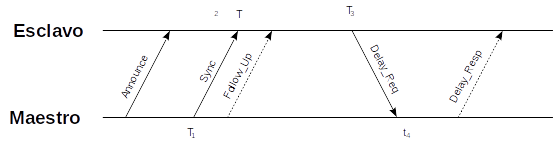
\includegraphics[width=0.7\linewidth]{imagenes/ptp_ts}
	\caption[Intercambio de mensajes para el algoritmo de \acrshort{ptp}]{La 
	figura muestra la secuencia de intercambio de mensajes 
	que se emplea en el algoritmo de \gls{ptp} para conseguir las 4 marcas de 
	tiempo necesarias en el cálculo del \textit{round-trip time} y del desfase.}
	\label{fig:ptpts}
\end{figure}

Para la clase de mensajes generales caben ser destacados los siguientes:

\begin{itemize}
	\item \textbf{Announce} \\
	Es el tipo de mensaje utilizado para informar al resto de los nodos acerca 
	del nodo que transmite (estado y características) además de quién es su 
	\gls{gm}. Son utilizados por el algoritmo \gls{bmc}.
	
	\item \textbf{Follow\_Up} \\
	Sirve para transmitir la marca de tiempo en la escala del maestro para la 
	emisión del mensaje \textit{Sync}.
	
	\item \textbf{Delay\_Resp} \\
	Análogo al anterior para el caso del mensaje \textit{Delay\_Req}.
	
	\item \textbf{Gestión y señalización} \\
	Se engloban mensajes para control y gestión de los relojes o para 
	transmitir información general de estado entre los nodos.
	
\end{itemize}


\subsection{Rendimiento}

Como se ha visto la esencia del mecanismo de sincronización de \gls{ptp} es 
similar al visto anteriormente en la sección de \gls{ntp}: se intercambian una 
serie de paquetes con marcas de tiempo entre dos nodos de la red para calcular 
el desfase entre sus relojes, entonces ¿cómo se consigue la mejora? La gran 
diferencia entre ambos protocolos es la inclusión en el primero del sellado de 
tiempo a nivel de \textit{hardware}. Cuando un paquete de tipo \gls{ptp} llega 
a un puerto, este genera un evento para que una lógica especial realice un 
sellado de tiempo de dicho paquete. Dicha lógica se encuentra entre la capa 
física (PHY) y la capa de enlace (MAC) del modelo \acrshort{osi} 
(\textit{\acrlong{osi}}). Este mecanismo evita la latencia que supone el 
procesamiento de los paquetes y el sellado de tiempo a nivel de 
\textit{software}. Otra diferencia significativa entre \gls{ntp} y \gls{ptp} se 
encuentra en la gestión de las colas de recepción/envío que son fuente de 
retardos no deterministas. Gracias al sellado con soporte \textit{hardware} y 
al tratamiento de los retardos ocasionados por las colas, \gls{ptp} consigue 
una precisión de decenas de nanosegundos con las técnicas más avanzadas 
actualmente \cite{5340221}.



